%!TEX TS-program = pdflatexmk

% Copyright 2019 Martin Scheidt (Attribution 4.0 International, CC-BY 4.0)
% You are free to copy and redistribute the material in any medium or format. You are free to remix, transform, and build upon the material for any purpose, even commercially. You must give appropriate credit, provide a link to the license, and indicate if changes were made. You may not apply legal terms or technological measures that legally restrict others from doing anything the license permits. No warranties are given.

\documentclass[
  % draft,
  paper=a4,
  version=3.25,
  pagesize=pdftex,
  twoside=false,
  DIV=12,
  headinclude=true,
  footinclude=false,
  toc=listof,
]{scrbook}

\def\ROOT{.}
%!TEX TS-program = pdflatexmk
%!TEX root = ../handbook.tex

% Copyright 2020 Martin Scheidt (Attribution 4.0 International, CC-BY 4.0)
% You are free to copy and redistribute the material in any medium or format. You are free to remix, transform, and build upon the material for any purpose, even commercially. You must give appropriate credit, provide a link to the license, and indicate if changes were made. You may not apply legal terms or technological measures that legally restrict others from doing anything the license permits. No warranties are given.

% --------[  Coding and Language  ]----------
\usepackage{scrhack}
\usepackage[utf8]{inputenc}
\usepackage[T1]{fontenc}
\usepackage[main=english,ngerman]{babel}
\usepackage{iflang}
\newcommand{\IfLanguage}[2]{\IfLanguageName{#1}{#2}{}}

% % --------[   revision history    ]----------
\usepackage{vhistory}
% % --------[ Creative Commons License ]-------
\usepackage[scale=1.5]{ccicons}

% --------[       drafting        ]----------
\usepackage{ifdraft}
\ifdraft{%
  \usepackage{draftwatermark}
  \SetWatermarkColor{base1!10}
}{}
%
\setlength{\marginparwidth }{2cm}
\usepackage[obeyDraft,textsize=footnotesize]{todonotes}

% --------[ Layout  ]-----------
\pretolerance=8000
\tolerance=9500
\hbadness=8000
\vbadness=10000
\displaywidowpenalty=10000
\clubpenalty=10000
\widowpenalty=10000
\usepackage{lmodern,microtype,mathptmx,courier}
\usepackage[scaled=0.92]{helvet}

\usepackage[
  automark,
  headsepline,
  draft=false
]{scrlayer-scrpage}

\pagestyle{scrheadings}

\usepackage{etoolbox}
\makeatletter
% \@addtoreset{chapter}{part} % reset chapter numbering for each part
\patchcmd{\scr@startchapter}{\if@openright\cleardoublepage\else\clearpage\fi}{}{}{} % remove page break after chapter
\makeatother

% -------[ Symbols ]---------
\usepackage{amsmath,amsthm}
\usepackage{xfrac} % provides slanted fractures with \sfrac{}{}
\usepackage{wasysym} % \permil
\usepackage{siunitx} % for SI-Units
\sisetup{
  per-mode=fraction,
  fraction-function=\sfrac
}

% -------[ Tables and Figures ]---------
\usepackage{graphicx}
\setkeys{Gin}{draft=false} % disable draft for graphicx to see pictures in draft-mode

\usepackage{booktabs,longtable,tabularx,ltxtable}

\usepackage{enumerate}
\usepackage{enumitem} % change numbering
\usepackage{tikz,adjustbox}
\usetikzlibrary{babel}

% -------[ costum commands ]---------
\newcommand{\TODO}[1]{\todo[linecolor=orange,backgroundcolor=orange!20,bordercolor=orange,inline,]{\textcolor{orange}{Todo:~}#1}}
\newcommand{\REWRITE}[1]{\todo[linecolor=magenta,backgroundcolor=magenta!20,bordercolor=magenta,noline]{\textcolor{magenta}{Rewrite:~}#1}}
\newcommand{\ADDFIGURE}[1]{\missingfigure[figcolor=white]{#1}}

\newcounter{task}[chapter] % reset couter <<task>> with each new chapter
\DeclareRobustCommand{\task}{\stepcounter{task}\bigskip\par\noindent{\normalfont\large\bfseries\IfLanguage{english}{Task~}\IfLanguage{ngerman}{Aufgabe~}\arabic{chapter}.\arabic{task}}\medskip\par\noindent}
\DeclareRobustCommand{\setup}{\bigskip\par\noindent{\normalfont\large\bfseries\IfLanguage{english}{Setup}\IfLanguage{ngerman}{Ausgangssituation}}\medskip\par\noindent}

\DeclareRobustCommand{\tikzfigure}[2][0.995\textwidth]{
  \begin{adjustbox}{width=#1}
    \begin{tikzpicture}[font=\sffamily]
      \input{\ROOT/figures/#2}
    \end{tikzpicture}
  \end{adjustbox}
}

%!TEX TS-program = pdflatexmk
%!TEX root = handbook.tex

% Copyright 2019 Martin Scheidt (Attribution 4.0 International, CC-BY 4.0)
% You are free to copy and redistribute the material in any medium or format. You are free to remix, transform, and build upon the material for any purpose, even commercially. You must give appropriate credit, provide a link to the license, and indicate if changes were made. You may not apply legal terms or technological measures that legally restrict others from doing anything the license permits. No warranties are given.

\usepackage[prefix=]{xcolor-solarized}
\definecolor{signalgreen}{RGB}{0,181,26}
\definecolor{signalyellow}{RGB}{255,230,0}
\definecolor{signalred}{RGB}{255,0,0}

%!TEX TS-program = pdflatexmk
%!TEX root = handbook.tex

% Copyright 2018 RailToolKit (Attribution 4.0 International, CC-BY 4.0)
% You are free to copy and redistribute the material in any medium or format. You are free to remix, transform, and build upon the material for any purpose, even commercially. You must give appropriate credit, provide a link to the license, and indicate if changes were made. You may not apply legal terms or technological measures that legally restrict others from doing anything the license permits. No warranties are given.

% -----------[ PDF linking ]----------------
\usepackage[
  pdftex,
  pdfpagelabels, % modify PDF page labels
  hyperindex,
  hyperfigures,
  bookmarksopen,
  bookmarksnumbered,
  draft=false,
  pageanchor=true, % Determines whether every page is given an implicit anchor at the top left corner
  %pagebackref, % Adds ‘backlink’ text to the end of each item in the bibliography, as a list of page numbers
  %linktocpage, % make page number, not text, be link on TOC, LOF and LOT
  breaklinks=true, % allow links to break over lines by making links over multiple lines into PDF links to the same target
  colorlinks=true, % Colors the text of links and anchors
  citecolor=violet, % Color for bibliographical citations in text
  linkcolor=base01, % Color for normal internal links
  urlcolor=blue, % Color for web links
]{hyperref} % PDF with a linked TableOfContent
\usepackage{bookmark} % Adding package bookmark improves bookmarks handling.
\usepackage{url}

% -------[ PDF Informations ]---------
\hypersetup{
  pdftitle={Traffic Flow in Railway Systems},
  pdfsubject={game based learning},
  pdfauthor={Martin Scheidt and contributers},
  pdfkeywords={railway, railroad, infrastructure, serious game},
}


\begin{document}

  \selectlanguage{english} % currently supported: english, ngerman

  %!TEX TS-program = pdflatexmk
%!TEX root = ../handbook.tex

% Copyright 2018 - 2022 Martin Scheidt (Attribution 4.0 International, CC-BY 4.0)
% You are free to copy and redistribute the material in any medium or format. You are free to remix, transform, and build upon the material for any purpose, even commercially. You must give appropriate credit, provide a link to the license, and indicate if changes were made. You may not apply legal terms or technological measures that legally restrict others from doing anything the license permits. No warranties are given.

\begin{titlepage}
%--------------------------------------------
  \thispagestyle{empty}
  \centering

  \vspace*{\fill}

  \bfseries\Huge Edugame Railway Operations

  \vspace*{\fill}

  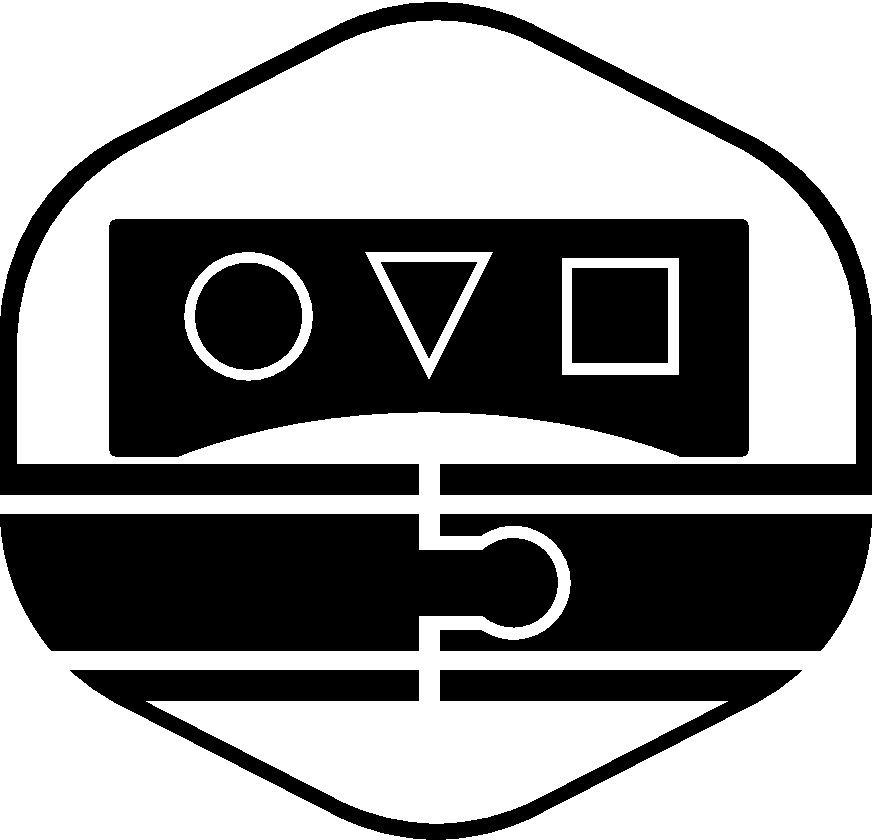
\includegraphics[keepaspectratio,width=0.3\textwidth]{../logo/logo.pdf}

  \vspace*{\fill}
  \vspace*{\fill}
  \vspace*{\fill}

  \normalfont\normalsize
  \IfLanguage{english}{``Gaming is an activity that cannot be taken seriously enough!''}
  \IfLanguage{ngerman}{``Spielen ist eine Tätigkeit, die man garnicht ernst genug nehmen kann!''} \\
  \flushright \emph{Jacques-Yves Cousteau}\par

  \vspace*{\fill}

  \flushleft PDF Download URL:\\
  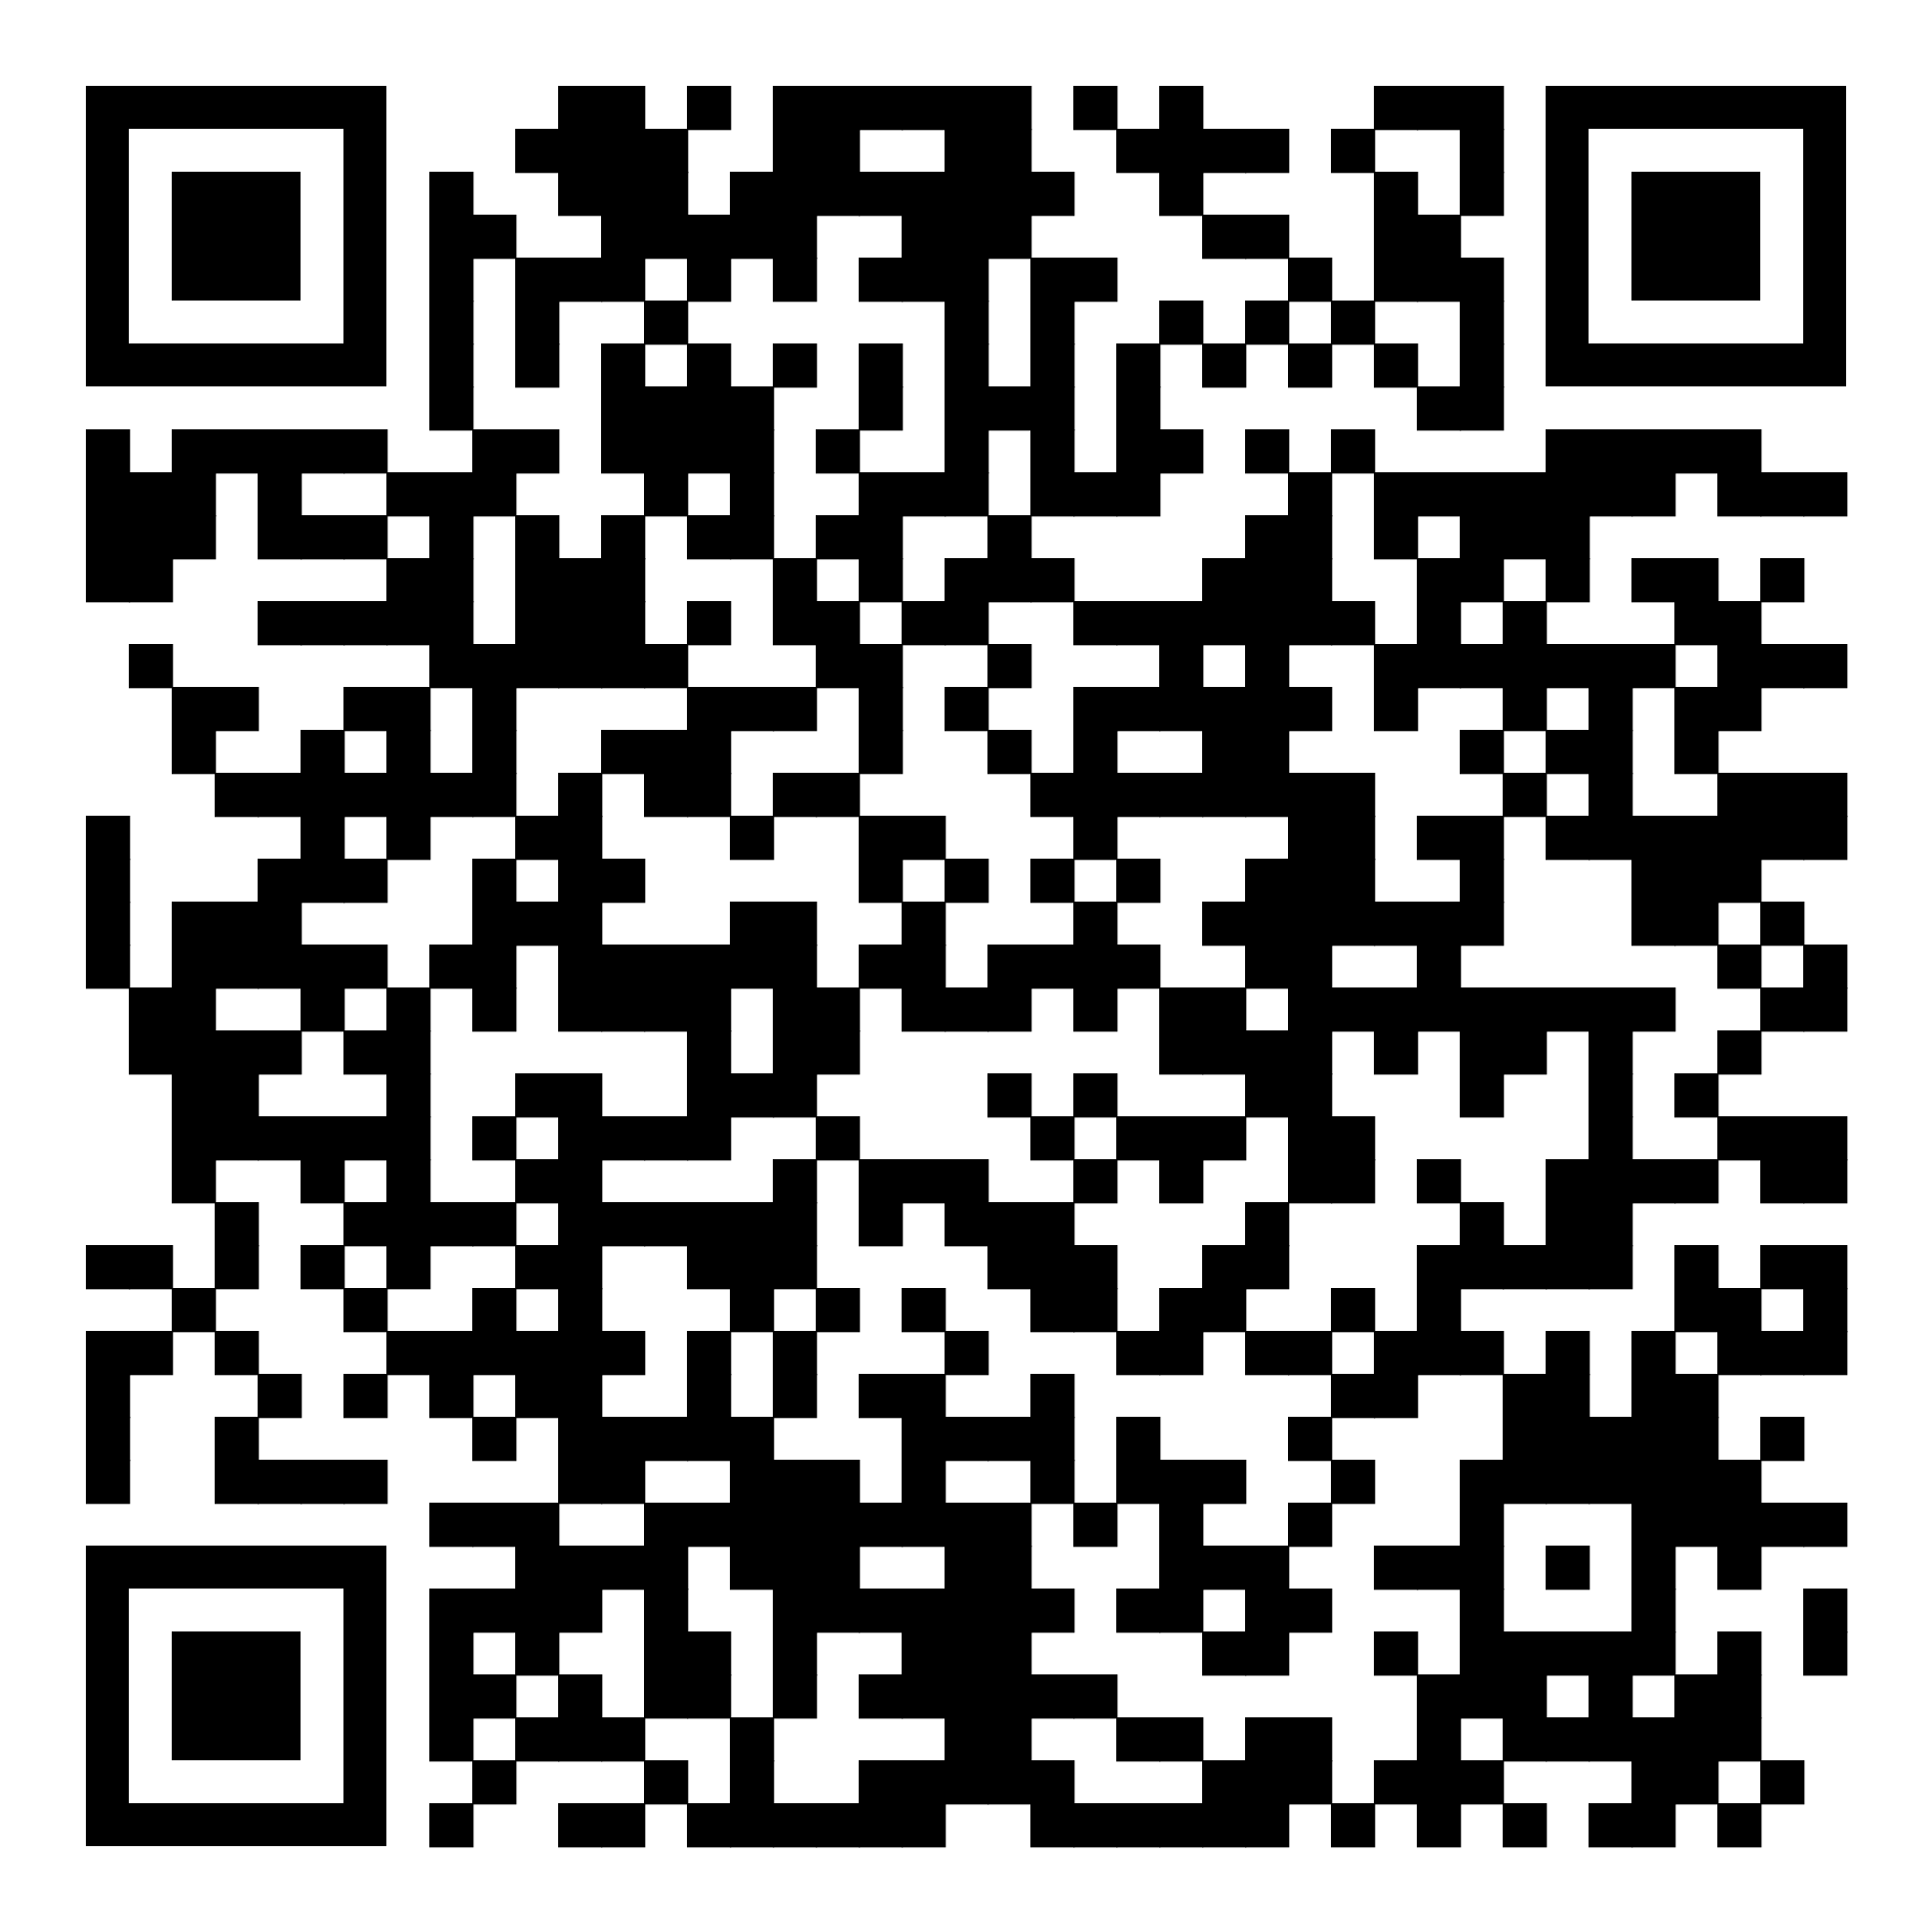
\includegraphics[keepaspectratio,width=0.2\textwidth]{figures/handbook_download_url.png} 

%--------------------------------------------
\end{titlepage}


  \tableofcontents
  \cleardoublepage

  %!TEX TS-program = pdflatexmk
%!TEX root = ../handbook.tex

% Copyright 2018 RailToolKit (Attribution 4.0 International, CC-BY 4.0)
% You are free to copy and redistribute the material in any medium or format. You are free to remix, transform, and build upon the material for any purpose, even commercially. You must give appropriate credit, provide a link to the license, and indicate if changes were made. You may not apply legal terms or technological measures that legally restrict others from doing anything the license permits. No warranties are given.
\chapter*{\IfLanguage{english}{Aim and Materials}\IfLanguage{ngerman}{Ziel und Materialien}}

\noindent
\IfLanguage{english}{The aim of the learning game is to simulate and experience the driving dynamics of trains in the context of block division. This requires:}
\IfLanguage{ngerman}{Ziel des Lernspieles ist die Fahrdynamik von Zügen im Zusammenhang mit Blockteilung zu simulieren und zu erfahren. Dafür wird benötigt:}
\begin{itemize}
  \IfLanguage{english}{
    \item two trains with different driving dynamics
    \item a track consisting of spaces
    \item train berths
    \item signals for block division
    \item if necessary, turnouts
  }
  \IfLanguage{ngerman}{
    \item zwei Züge mit unterschiedlicher Fahrdynamik
    \item eine Strecke, bestehend aus Spielfeldern
    \item Halteplätze für die Züge
    \item Signale für die Blockteilung
    \item ggf. Weichen
  }
\end{itemize}
\IfLanguage{english}{Real continuous dimensions time ($t$) and distance ($s$) are assigned to discrete units of rounds ($t$) and spaces ($s$).
Thus, the simulation is round-based in order to imitate the steps of a computer.}
\IfLanguage{ngerman}{Reale kontinuierliche Größen Zeit ($t$) und Strecke ($s$) werden dabei in diskrete Einheiten von Runden ($t$) und Felder ($s$) eingeteilt.
Die Simulation erfolgt also Rundenbasiert, um im Schrittverfahren einen Computer nachzuahmen.}

\vspace*{\fill}

\IfLanguage{english}{
  {\noindent\large Version \vhCurrentVersion\ from \vhCurrentDate } \\[0.3cm]
  \ccLogo \ccAttribution ~This work is licensed under a Creative Commons License (CC BY 4.0).
}
\IfLanguage{ngerman}{
  {\noindent\large Version \vhCurrentVersion\ vom \vhCurrentDate } \\[0.3cm]
  \ccLogo \ccAttribution ~Dieses Werk steht unter der Creative Commons Lizens (CC BY 4.0).
}

  \cleardoublepage

  \setcounter{part}{1}
  %!TEX TS-program = pdflatexmk
%!TEX root = ../handbook.tex

% Copyright 2018 RailToolKit (Attribution 4.0 International, CC-BY 4.0)
% You are free to copy and redistribute the material in any medium or format. You are free to remix, transform, and build upon the material for any purpose, even commercially. You must give appropriate credit, provide a link to the license, and indicate if changes were made. You may not apply legal terms or technological measures that legally restrict others from doing anything the license permits. No warranties are given.

\part{\IfLanguage{english}{Challenges}\IfLanguage{ngerman}{Aufgaben}}
  
\chapter{\IfLanguage{english}{First Stage}\IfLanguage{ngerman}{Erste Stufe}}
  \section{\IfLanguage{english}{Introduction to Driving Dynamics}\IfLanguage{ngerman}{Einführung Fahrdynamik}}
    \setup
      \begin{itemize}
        \IfLanguage{english}{
          \item A single train,
          \item Line with fields    $-2$ to $36$,
          \item Platform A at field $-2$ to $0$,
          \item Platform B at field $13$ to $15$,
          \item Platform C at field $34$ to $36$.
        }
        \IfLanguage{ngerman}{
          \item ein Zug,
          \item Strecke mit Feldern $-2$ bis $36$,
          \item Bahnsteig A am Feld $-2$ bis $0$,
          \item Bahnsteig B am Feld $14$ bis $15$,
          \item Bahnsteig C am Feld $34$ bis $36$.
        }
      \end{itemize}
    \task
      \IfLanguage{english}{ The train (on field $0$ towards $36$) stands still and has its shift lever at \SI{0}{\kilo\metre\per\hour}.}
      \IfLanguage{ngerman}{Der Zug (auf Feld $0$ in Richtung $36$) steht und hat seinen Schalthebel auf \SI{0}{\kilo\metre\per\hour}.}
      \begin{enumerate}[label=\alph*)]
        \IfLanguage{english}{
          \item If the train accelerates as much as possible, which field can it get to in \emph{nine} laps?
          \item How many laps are minimally needed, if the train stops at every station?
        }
        \IfLanguage{ngerman}{
          \item Wenn der Zug maximal beschleunigt, bis zu welchen Feld gelangt er in \emph{neun} Runden?
          \item Wie viele Runden benötigt man minimal, wenn der Zug in jedem Bahnhof halten soll?
        }
      \end{enumerate}
      \IfLanguage{english}{Note the solution steps in a protocol!}
      \IfLanguage{ngerman}{Notiere die Lösungschritte in einem Protokoll!}
      % \begin{center}
      %   \IfLanguage{english}{Example for a protocol:}
      %   \IfLanguage{ngerman}{Beispiel für ein Protokoll:}
      %   \\
      %   %!TEX TS-program = pdflatexmk
%!TEX root = ../handbook.tex

% Copyright 2018 Martin Scheidt (ISC license)
% Permission to use, copy, modify, and/or distribute this file for any purpose with or without fee is hereby granted, provided that the above copyright notice and this permission notice appear in all copies.

\begin{tabular}{cccc|c}
  \toprule
  \IfLanguage{english}{
  Round   & curent                      & (1. Step)   & current position  & (2. Step)                     \\
          & speed                       & Move by     & head of train     & shift lever at                \\

  }
  \IfLanguage{ngerman}{
  Runde   & aktuelle                    & (1. Schritt)& aktuelle          & (2. Schritt)                  \\
          & Geschwindigkeit             & Bewegen um  & Position Zugspitze& Schalthebel auf               \\
  }
  \hline
  \IfLanguage{english}{
  $1$     & \SI{0}{\kilo\metre\per\hour}& $0$ fields  & field $0$         & \SI{40}{\kilo\metre\per\hour} \\
  }
  \IfLanguage{ngerman}{
  $1$     & \SI{0}{\kilo\metre\per\hour}& $0$ Felder  & Feld $0$          & \SI{40}{\kilo\metre\per\hour} \\
  }
  \hline
  $2$     & $\cdots$                    &             &                   &                               \\
  \hline
  $\vdots$&                             &             &                   &                               \\
  \hline 
          &                             &             &                   &                               \\
  \bottomrule
\end{tabular}

      % \end{center}
    \task
      \IfLanguage{english}{ The train (on field $0$ towards $37$) just passes through the first station and has its shift lever on maximum speed.}
      \IfLanguage{ngerman}{Der Zug (auf Feld $0$ in Richtung $37$) fährt gerade durch den ersten Bahnhof durch und hat seinen Schalthebel auf der maximalen Geschwindigkeit.}
      \begin{enumerate}[label=\alph*)]
        \IfLanguage{english}{
          \item How many fields does the train need to come to a stop?
          \item How many laps are needed if the train shall leave the track completely without stopping?
        }
        \IfLanguage{ngerman}{
          \item Wie viele Felder braucht der Zug, bis er zum Stehen gekommen ist?
          \item Wie viele Runden benötigt man, wenn der Zug ohne Halt die Strecke vollständig verlassen soll?
        }
      \end{enumerate}
      
  \newpage

  \section{\IfLanguage{english}{Sight and Braking Distance}\IfLanguage{ngerman}{Sicht- und Bremsweg}}
    \setup
      \IfLanguage{english}{Unknown line with different visibility conditions:}
      \IfLanguage{ngerman}{Unbekannte Strecke mit verschiedenen Sichtverhältnissen:}
      \\[0.5cm]
      %!TEX TS-program = pdflatexmk
%!TEX root = ../handbook.tex

% Copyright 2018 Martin Scheidt (ISC license)
% Permission to use, copy, modify, and/or distribute this file for any purpose with or without fee is hereby granted, provided that the above copyright notice and this permission notice appear in all copies.

\begin{tabular}{rl}
  \toprule
  \IfLanguage{english}{
    Visibility      & Sight in fields   \\
  }
  \IfLanguage{ngerman}{
    Sichtverhältnis & Sicht in Feldern  \\
  }
  \hline
  \IfLanguage{english}{
    Very good       & 3                 \\
    Normal          & 2                 \\
    Bad             & 1                 \\
  }
  \IfLanguage{ngerman}{
    Sehr gut        & 3                 \\
    Normal          & 2                 \\
    Schlecht        & 1                 \\
  }
  \bottomrule
\end{tabular}

    \task
      \begin{enumerate}[label=\alph*)]
        \IfLanguage{english}{
          \item What is the maximum speed for the train with very good visibility in order to stop in front of an obstacle in time?
          \item How many laps does it take to get safely to a station $12$ fields away under normal visibility conditions?
          \item How many fields far would you have to be able to see in order to drive \SI{160}{\kilo\metre\per\hour}?
        }
        \IfLanguage{ngerman}{
          \item Wie schnell kann der Zug bei sehr gutem Sichtverhältnis maximal Fahren um vor einem Hindernis rechtzeitig anzuhalten?
          \item Wie viele Runden benötigt man minimal, um gefahrlos bei normalen Sichtverhältnissen in einem $12$ Felder entfernten Bahnhof zu gelangen?
          \item Wie viele Felder weit müsste man sehen können, um \SI{160}{\kilo\metre\per\hour} fahren zu können?
        }
      \end{enumerate}

\chapter{\IfLanguage{english}{Second Stage}\IfLanguage{ngerman}{Zweite Stufe}}
  \section{\IfLanguage{english}{Block Segmentation}\IfLanguage{ngerman}{Blockteilung}}
    \setup
      \IfLanguage{english}{One train and any length of line, with at least 3 complete blocks.
      A block consists of: visual point, distant signal, main signal, signal clearing point and clearing distance.}
      \IfLanguage{ngerman}{Ein Zug und eine beliebig lange Strecke, mit mindestens 3 vollständigen Blöcken.
      Ein Block besteht aus: Sichtpunkt, Vorsignal, Hauptsignal, Signalzugschlussstelle und Räumweg.}
    \task
      \begin{enumerate}[label=\alph*)]
        \IfLanguage{english}{
          \item Place the distant and main signals so that \SI{160}{\kilo\metre\per\hour} can be driven and bad visibility does not lead to impairment!
          \item How many laps is a block occupied with a train run minimally (complete blocking time)?
        }
        \IfLanguage{ngerman}{
          \item Platziere die Vor- und Hauptsignale mindestens so, dass \SI{160}{\kilo\metre\per\hour} gefahren werden kann und schlechte Sichtverhältnisse nicht zur Beeinträchtigung führt!
          \item Wie viele Runden ist ein Block mit einer Zugfahrt minimal belegt (vollständige Sperrzeit)?
        }
      \end{enumerate}

  \section{\IfLanguage{english}{Traffic Flow}\IfLanguage{ngerman}{Verkehrsfluss}}
    \setup
      \begin{itemize}
        \IfLanguage{english}{
          \item Two different trains with different train dynamics.
          \item A track with at least 3 complete blocks.
          \item Am Anfang der Strecke brechen Züge ein. Am Ende der Strecke brechen Züge aus. Die Infrastruktur vor und nach der Strecke wird vernachlässigt.
        }
        \IfLanguage{ngerman}{
          \item Zwei verschiedene Züge mit unterschiedlicher Fahrdynamik.
          \item Eine Strecke, mit mindestens 3 vollständigen Blöcken.
          \item Am Anfang der Strecke brechen Züge ein. Am Ende der Strecke brechen Züge aus. Die Infrastruktur vor und nach der Strecke wird vernachlässigt.
        }
      \end{itemize}
    \task
      \begin{enumerate}[label=\alph*)]
        \IfLanguage{english}{
          \item How many laps are needed from the first train breaking in to the second train leaving if both trains are to run unimpeded and the \emph{fast} runs in front of the \emph{slow} train?
          \item How many laps are needed from the first train breaking in to the second train leaving if both trains are to run unimpeded and the \emph{slow} runs in front of the \emph{fast} train?
        }
        \IfLanguage{ngerman}{
          \item Wie viele Runden werden benötigt vom Einbruch des ersten Zuges bis zum verlassen des zweiten Zuges, wenn beide Züge behinderungsfrei fahren sollen und der \emph{schnelle} vor dem \emph{langsamen} Zug fährt?
          \item Wie viele Runden werden benötigt vom Einbruch des ersten Zuges bis zum verlassen des zweiten Zuges, wenn beide Züge behinderungsfrei fahren sollen und der \emph{langsame} vor dem \emph{schnellen} Zug fährt?
        }
      \end{enumerate}

  \cleardoublepage
  \appendix
  %!TEX TS-program = pdflatexmk
%!TEX root = ../handbook.tex

% Copyright 2020 Martin Scheidt (Attribution 4.0 International, CC-BY 4.0)
% You are free to copy and redistribute the material in any medium or format. You are free to remix, transform, and build upon the material for any purpose, even commercially. You must give appropriate credit, provide a link to the license, and indicate if changes were made. You may not apply legal terms or technological measures that legally restrict others from doing anything the license permits. No warranties are given.

\newcommand{\MS}{Martin Scheidt}
\newcommand{\FN}{Felix Nebel}
\newcommand{\LG}{Lukas Gruber}
\newcommand{\LP}{Leonhard Pelster}
\newcommand{\SZ}{Stephan Zieger}
\newcommand{\LE}{Laura Enders}
\begin{versionhistory}
  %\vhEntry{<Version>}{<Date>}{<Author1>|<Author2>|...}{<Changes>}
  \vhEntry{0.1}{2018-04-17}{MS|FN|LG}{
    \IfLanguage{ngerman}{Ersten Prototyp mit Fahrdynamik erstellt}
    \IfLanguage{english}{First prototype created with driving dynamics}
  }
  \vhEntry{0.2}{2018-05-15}{MS|LG}{
    \IfLanguage{ngerman}{Lehrspiel mit Blocklogik erweitert}
    \IfLanguage{english}{Educational game with block logic extended}
  }
  \vhEntry{0.3}{2018-09-03}{MS}{
    \IfLanguage{ngerman}{Handbuch erstellt}
    \IfLanguage{english}{Handbook created}
  }
  \vhEntry{0.3.1}{2018-10-17}{MS}{
    \IfLanguage{ngerman}{Handbuch mit neutralem Design}
    \IfLanguage{english}{Handbook with neutral design}
  }
  \vhEntry{0.4}{2018-11-16}{MS|LE|SZ}{
    \IfLanguage{ngerman}{Übersetzung ins Englische}
    \IfLanguage{english}{Translation into english}
  }
  \vhEntry{0.5}{2019-03-29}{MS}{
    \IfLanguage{ngerman}{Kleinere Verbesserungen und Bastelbögen}
    \IfLanguage{english}{Minor improvements and craft sheets}
  }
  \vhEntry{0.5.1}{2019-03-29}{MS}{
    \IfLanguage{ngerman}{Anpassung der Streckenlänge und Aufgaben}
    \IfLanguage{english}{Adaptation of track length and tasks}
  }
  \vhEntry{0.6}{2019-05-20}{MS}{
    \IfLanguage{ngerman}{Fahrstraßen und Fahrstraßenverschluss hinzugefügt}
    \IfLanguage{english}{Added routes and route locking}
  }
  \vhEntry{0.6.1}{2019-08-26}{MS|LP}{
    \IfLanguage{ngerman}{Aufgaben für Fahrstraßen erweitert}
    \IfLanguage{english}{Extended tasks for routes}
  }
  \vhEntry{0.7}{2019-09-09}{MS|LP}{
    \IfLanguage{ngerman}{Spielmechanik mit Aufgaben und Abbildungen überarbeitet}
    \IfLanguage{english}{reworking of game mechanics together with tasks and figures}
  }
  \vhEntry{0.7.1}{2019-09-17}{MS}{
    \IfLanguage{ngerman}{Signale fürs Links- und Rechtsfahren angepasst}
    \IfLanguage{english}{Adapted signals for left- and right-hand traffic}
  }
  \vhEntry{0.7.2}{2019-09-20}{MS}{
    \IfLanguage{ngerman}{Aufgaben aus Version 0.6.1 in englisch ergänzt}
    \IfLanguage{english}{Supplemented tasks in English from version 0.6.1}
  }
  \vhEntry{1.0}{2020-06-20}{LP|MS}{
    \IfLanguage{ngerman}{Überarbeitung und Neukonzeption}
    \IfLanguage{english}{Revision and new conceptual design}
  }
\end{versionhistory}

  \vhListAllAuthorsLongWithAbbrev

\end{document}